% Chapter 4

\chapter{Internship Subject} % Main chapter title

\label{Chapter3} % For referencing the chapter elsewhere, use \ref{Chapter3}

%----------------------------------------------------------------------------------------

% Define some commands to keep the formatting separated from the content
%\newcommand{\keyword}[1]{\textbf{#1}}
%\newcommand{\tabhead}[1]{\textbf{#1}}
%\newcommand{\code}[1]{\texttt{#1}}
%\newcommand{\file}[1]{\texttt{\bfseries#1}}
%\newcommand{\option}[1]{\texttt{\itshape#1}}

%----------------------------------------------------------------------------------------

\section{Problematics}

As I said in the previous parts, \iBubble{} includes a visual tracking system, \keyword{CMT}, to \emph{autonomously} follow divers underwater. This system currently uses \emph{openCV} libraries at a rate of \textbf{30 fps}. This speed can be improved using \emph{CUDA} technology. These feat{}s are only available on \keyword{BtB} versions of \iBubble{} fitted with \emph{Nvidia's Jetson embedded board}.

\keyword{BtC} versions of the drone uses \rasp{} in spite of the current \emph{Nvidia Graphics Card} wich means that \emph{CUDA} is no longer available because \vc{} is not designed with this technology.

As a consequence, \vc{} is not used so the whole tracking system is running only on the \cpu{} and the system rate drops to \textbf{7 fps}.

The more time-consuming part of the \keyword{CMT} is the \flow{} computation. This is a fundamental tracking algorithm in Computer Vision. It uses \keyword{Gradient Descent} and \keyword{Pyramid} algorithms to get the displacement of the points of interest between two frames.

Therefore if we want to use the computing power of the \vc{}, it is compulsory to make our own implementation of the \flow{} on \rasp, that was my internship subject.

The main difficulty is that there is no official \api{} released by \textsc{Broadcom}. To compute the \flow{} on \rasp, it was to necessary to follow the same steps as in Chapter~\ref{Chapter2}, namely:
\begin{itemize}
	\item write \code{code-to-execute} on \keyword{GPU} -- in \option{assembly language}
	\item parse this \code{code-to-execute} with \keyword{assembly parser} -- \file{qpu-asm.cpp}
	\item write a \code{driver program} for the \keyword{CPU} -- in \option{c-language}
	\item include this \api{} in a \option{C++} project -- \keyword{CMT} is written in \option{C++}
\end{itemize}

%----------------------------------------------------------------------------------------

\section{Optical Flow}

\subsection{Definition}

Within \iBubble{} visual tracking system - \keyword{CMT} - \flow{} is the displacement of points of interest - called \feat{}s - between two consecutive frames from a video.

Computing \emph{optical flow} between two consecutive frames involves the following steps:
\begin{itemize}
	\item detect \feat{}s on first image -- Figure~\ref{initFeaturesFig}
	\item find the next \feat{}s positions on the second image -- Figure~\ref{secondFeaturesFig}
	\item compute \emph{displacemnt} for each \feat{}s -- Figure~\ref{opticalFlowFig}
\end{itemize}


\begin{figure}[!htbp]
	\centering
	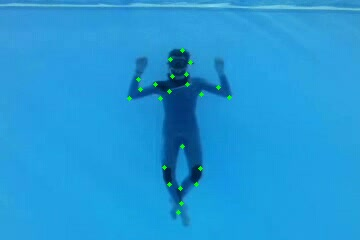
\includegraphics[width=0.5\textwidth]{plongeurInitFeatures}
	\caption{First frame of a diving video with the initial set of \feat{}s}
	\label{initFeaturesFig}
\end{figure}
\FloatBarrier



\begin{figure}[!htbp]
	\centering
	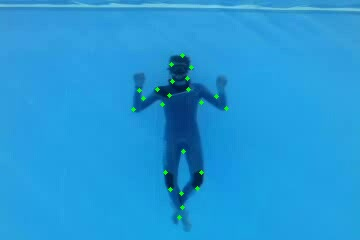
\includegraphics[width=0.5\textwidth]{plongeurNextFeatures}
	\caption{Second frame of a diving video with new \feat{}s positions}
	\label{secondFeaturesFig}
\end{figure}
\FloatBarrier



\begin{figure}[!htbp]
	\centering
	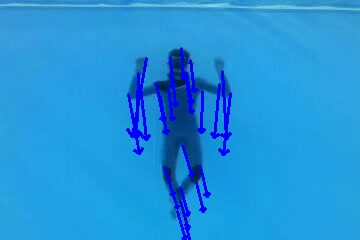
\includegraphics[width=0.5\textwidth]{plongeurOpticalFlow}
	\caption{Optical flow for the initial set of \feat{}s -- \small{norm of the \textcolor{blue}{blue vectors} is overstated for better visualization}}
	\label{opticalFlowFig}
\end{figure}
\FloatBarrier

\emph{Optical flow} can be viewed as a \emph{vector field} representing \feat{}s displacement between two consecutive frames. It is used to do object recognition, tracking or movement detection. In \iBubble, \emph{optical flow} is compute within \keyword{CMT} to achieve diver \emph{autonomous tracking and following}.\par


\subsection{Images encoding}

As I mentioned in~\ref{Matrices}, frames from the \rasp's camera (Figures~\ref{initFeaturesFig} to ~\ref{opticalFlowFig}) are \option{row major float-matrices}. More specifically, a frame is a ($240\times 360$) pixel array:

\begin{figure}[!htbp]
\[
\begin{bmatrix}

pixel_{0,0} & pixel_{0,1} & \ldots & \ldots & \ldots & pixel_{0,359}\\

pixel_{1,0} & \ddots & \ldots & \ldots & \ldots & pixel_{1,359}\\

\vdots & \ldots & \ddots & \ldots & \ldots & \vdots\\

\vdots & \ldots & \ldots & \cellcolor{yellow}{feature_{x,y}} & \ldots & \vdots\\

\vdots & \ldots & \ldots & \ldots & \ddots & \vdots\\

pixel_{239,0} & \ldots & \ldots  & \ldots & \ldots & pixel_{239,359}

\end{bmatrix}_{240\times 360}
\]
\caption{Frame from camera: two-dimensionnal pixel array}
\label{frameFig}
\end{figure}
\FloatBarrier

Moreover, \flow{} algorithm uses \emph{grayscale} images:

\begin{itemize}
	\item each $pixel_{x,y}$ is encoded as \option{32-bit float}
	\item stored at @$pixel_{x,y}$ address
	\item @$pixel_{x,y}$ is a \option{32-bit integer} -- Appendice~\ref{AppendixB}
\end{itemize}


From the shared RAM point of view, a frame is a contiguous array:
\begin{figure}[h]
\begin{center}
\begin{tabular}{|c|c|c|}

	\hline
	\begin{bf}$\text{@pixel}_\text{{x,y}}$\end{bf} & \begin{bf}offset\end{bf} & \begin{bf}$\text{@pixel}_\text{{x,y}}$\end{bf} \\[10pt]

	\hline
	@$pixel_{0,0}$ & @$pixel_{0,0}$ & $pixel_{0,0}$ \\

	\hline
	@$pixel_{0,1}$ & @$pixel_{0,0} + 4$ & $pixel_{0,1}$ \\

	\hline
	\vdots & \vdots & \vdots \\

	\hline
	@$pixel_{0,359}$ & @$pixel_{0,0} + 359\times 4$ & $pixel_{0,359}$ \\

	\hline
	@$pixel_{1,0}$ & @$pixel_{0,0} + 1\times 360$ & $pixel_{1,0}$ \\

	\hline
	@$pixel_{1,1}$ & @$pixel_{0,0} + 1\times 360 + 1\times 4$ & $pixel_{1,1}$ \\

	\hline
	\vdots & \vdots & \vdots \\

	\hline
	\rowcolor{yellow}@$pixel_{x,y}$ & @$pixel_{0,0} + x\times 360 + y\times 4$ & $pixel_{x,y}$ \\

	\hline
	\vdots & \vdots & \vdots \\

	\hline
	@$pixel_{x,y}$ & @$pixel_{0,0} + 239\times 360 + 359\times 4$ & $pixel_{239,359}$ \\

	\hline

\end{tabular}
\end{center}
\caption{Contiguous Array in Memory}
\end{figure}
\FloatBarrier

As a result to access particular $pixel_{x,y}$ value with the \qpu, we must pass 3 parameters to the \vc's \keyword{TMU}:
\begin{itemize}
	\item @$pixel_{0,0}$ -- starting address of the frame in the \emph{VC CPU Bus Addresses}
	\item $x$ -- pixel row number
	\item $y$ -- pixel coloumn number
\end{itemize}

Within a frame, a \feat{} is a specific $pixel$ with specific $(x,y)$ numbers (Figure~\ref{frameFig}). To know the \option{32-bit float value} of $feature_{x,y}$, we must pass those 3 parameters to the \keyword{TMU}.


\subsection{Parameters, Notations and Expected Outcomes}


\subsubsection{Parameters}\label{parameters}

Before invoking the \flow{} computation, the \emph{tracking system} must provide three parameters to the \vc:

\begin{itemize}
	\item first frame data -- must be a pointer to the first pixel $\textcolor{blue}{firstFrame_{0,0}}$
	\item 30 $feature_{x,y}$ positions -- must be a pointer to an integer array: \file{int} $featuresArray[2][30]$
	\item second frame data -- must be a pointer to the first pixel $\textcolor{red}{secondFrame_{0,0}}$
\end{itemize}


\subsubsection{Notations}

All notations are summarized on Figure~\ref{framesWindowFig}.

A pixel from first frame will be noted $\textcolor{blue}{firstFrame_{x,y}}$.\\
A pixel from second frame will be noted $\textcolor{red}{secondFrame_{x,y}}$.\\
A pixel from window in firstFrame will be noted $\textcolor{blue}{firstWindow_{x,y}}$.\\
A pixel from window in secondFrame will be noted $\textcolor{red}{secondWindow_{x,y}}$.\\
A feature \keyword{row number} will be noted $\textcolor{blue}{x_{1}}$ on \textcolor{blue}{firstFrame} and $\textcolor{red}{x_{2}}$ on \textcolor{red}{secondFrame}.\\
A feature \keyword{column number} will be noted $\textcolor{blue}{x_{1}}$ on \textcolor{blue}{firstFrame} and $\textcolor{red}{x_{2}}$ on \textcolor{red}{secondFrame}.\\
Finally, the \keyword{same feature} will be noted $feature_{\textcolor{blue}{y_{1},y_{1}}}$ on \textcolor{blue}{firstFrame} and $feature_{\textcolor{red}{x_{1},y_{1}}}$ on \textcolor{red}{secondFrame}.

\subsubsection{Expected Outcomes}

The expected results of the \flow{} algorithm are written Figure~\ref{framesWindowFig}. For each \feat{}, the \vc{} must compute:
\begin{itemize}
	\item \textbf{$d_{x}$} -- the feature displacement along the row axis measured in pixel: $\textcolor{red}{x_{2}}-\textcolor{blue}{x_{1}}$
	\item \textbf{$d_{y}$} -- the feature displacement along the column axis measured in pixel: $\textcolor{red}{y_{2}}-\textcolor{blue}{y_{1}}$
\end{itemize}

So the \flow{} program will return a \file{float} $displacementsArray[2][30]$ containing:
\begin{itemize}
	\item 30 $d_{x}$ \option{float values} -- one for each feature
	\item 30 $d_{y}$ \option{float values} -- one for each feature
\end{itemize}

This is the \flow{} between two consecutive frames for 30 \feat{}s.


\subsubsection{Summary}

To summarize the \flow{} computation between two consecutive frames for each feature on \vc:
\begin{itemize}
	\item inputs:
		\begin{itemize}
			\item $\textcolor{blue}{firstFrame_{0,0}}$ pointer
			\item $\textcolor{red}{secondFrame_{0,0}}$ pointer
			\item \file{int} $featuresArray[2][30]$
		\end{itemize}
	\item outputs: \file{float} $displacementsArray[2][30]$
\end{itemize}

\begin{figure}[!htbp]
	\centering
	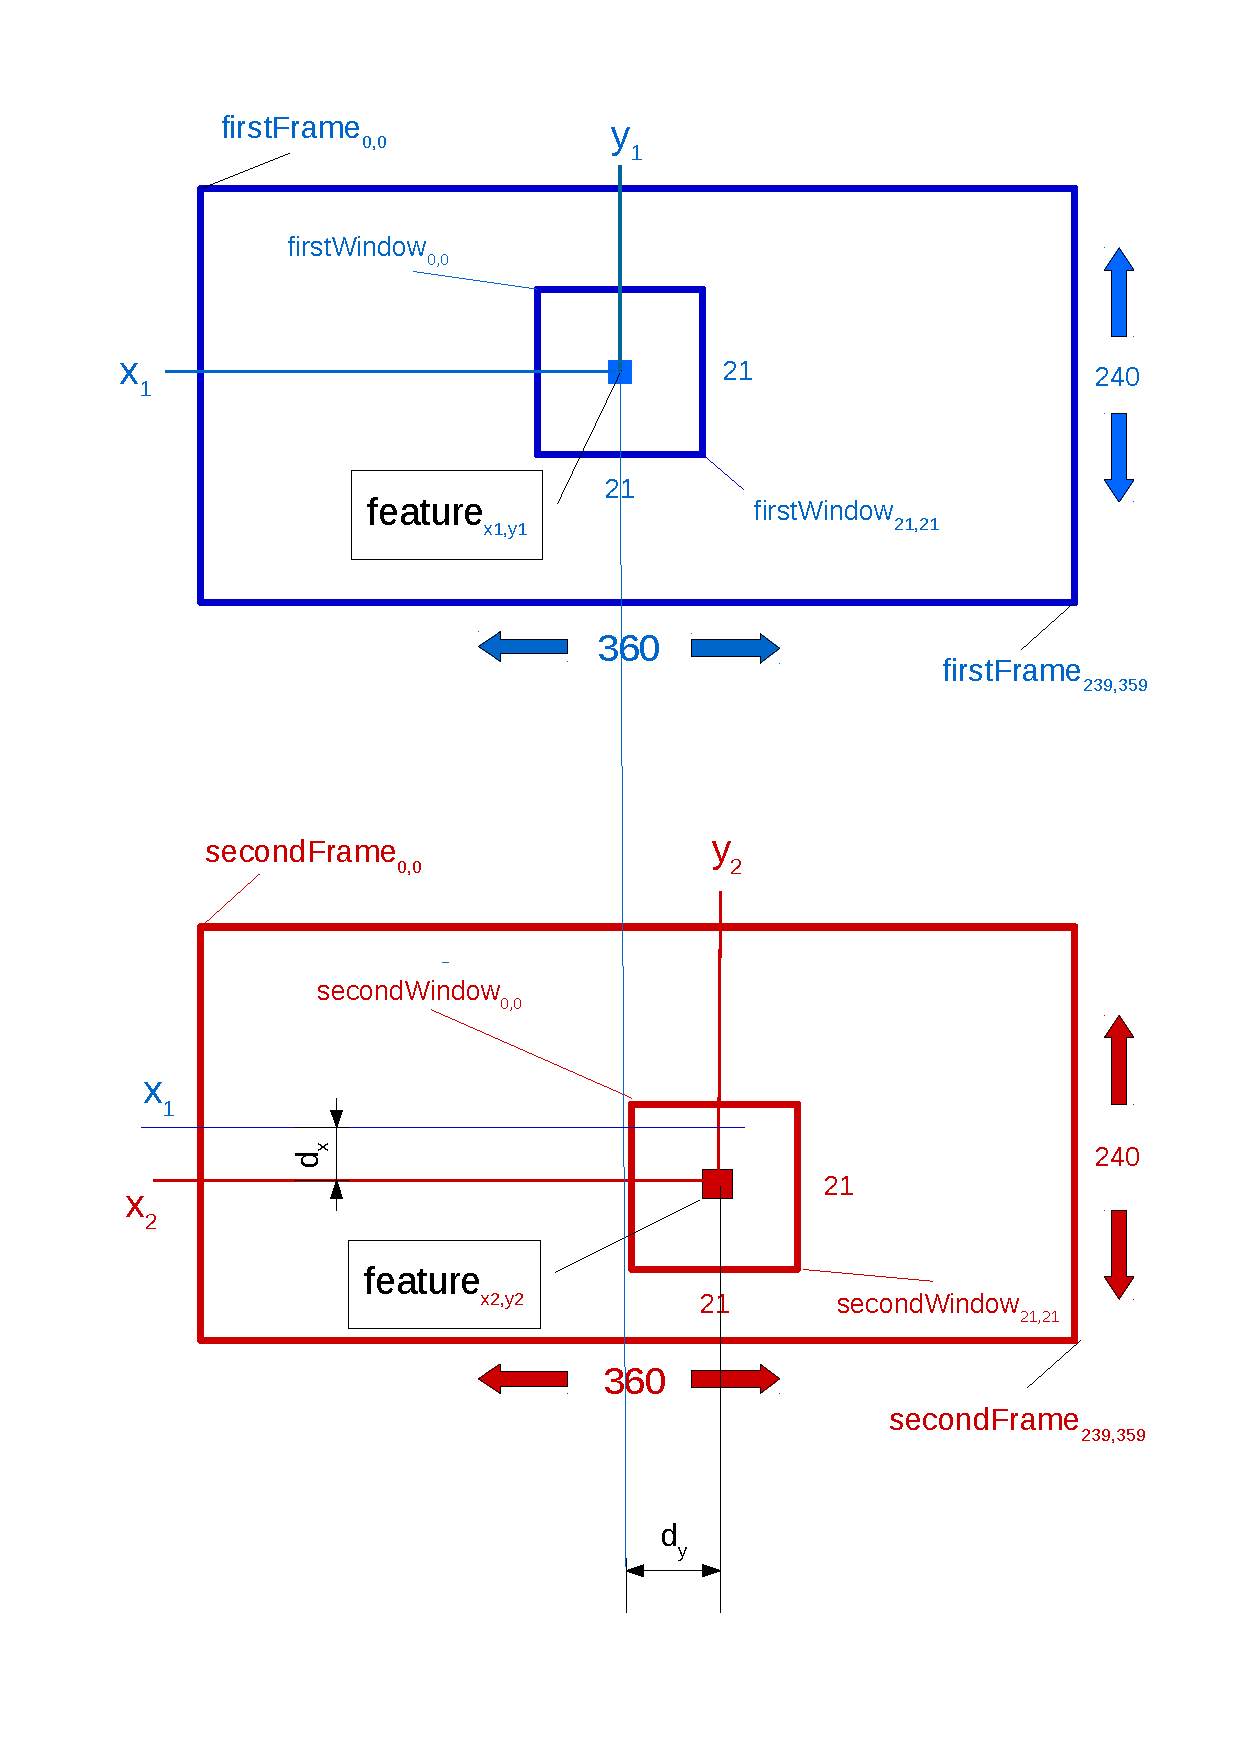
\includegraphics[width=0.8\textwidth]{framesWindow}
	\caption{Optical flow between \textcolor{blue}{first frame} and \textcolor{red}{second frame} for one feature}
	\label{framesWindowFig}
\end{figure}
\FloatBarrier

%----------------------------------------------------------------------------------------

\section{Lucas-Kanade method}

There are several ways to compute \flow{}. Camille selected \keyword{Lucas-Kanade} method to be implemented on \vc.

The \emph{vision tracking} algorithm detects \keyword{30} feat{}s on each frame from the camera. Thus, our \emph{homemade} algorithm must compute \flow{} for these 30 feat{}s between two consecutive frames.

Although there are 30 feat{}s, I will present the Lucas-Kanade method for one \feat{}, $feature_{x,y}$. The processing is the same for the rest of the feat{}s.

For the rest of this section, keep in mind Figure~\ref{framesWindowFig}.

\subsection{First Frame Processing}\label{gradientProcessing}

When \vc{} gets $\textcolor{blue}{firstFrame_{0,0}}$, \file{int} $featuresArray[2][30]$ and $\textcolor{red}{secondFrame_{0,0}}$ he starts processing the first frame.

The goal is to get 4 values per \feat{}:
\begin{itemize}
	\item $G_{XX}$ -- vertical gradient of the feature
	\item $G_{YY}$ -- horizontal gradient of the feature
	\item $G_{XY}$ -- cross gradient of the feature
	\item $det = \frac{1}{G_{XX}G_{YY}-G_{XY}G_{XX}}$
\end{itemize}

As shown in Figure~\ref{framesWindowFig}, we use a $21\times21$ \option{pixel window} around the feature:

$$G_{XX} = \sum_{i=1}^{21}\sum_{j=1}^{21} grad_{x}[i,j]^{2}$$
$$G_{YY} = \sum_{i=1}^{21}\sum_{j=1}^{21} grad_{y}[i,j]^{2}$$
$$G_{XY} = \sum_{i=1}^{21}\sum_{j=1}^{21} grad_{x}[i,j]\times grad_{y}[i,j]$$

Where, for a pixel element - $firstWindow_{i,j}$ -  of the window:
$$grad_{x}[i,j] = \frac{\textcolor{blue}{firstWindow_{i+1,j}} - \textcolor{blue}{firstWindow_{i-1,j}}}{2}$$
$$grad_{y}[i,j] = \frac{\textcolor{blue}{firstWindow_{i,j+1}} - \textcolor{blue}{firstWindow_{i,j-1}}}{2}$$


\subsection{Displacement computation}

To compute the feature displacement, we use the following algorithm:

\begin{figure}[!htbp]
\begin{algorithmic}
	\ForAll {$\textcolor{blue}{firstWindow_{i,j}}$ and $\textcolor{red}{secondWindow_{i,j}}$}

	\State $diff\_frames = \textcolor{blue}{firstWindow_{i,j}} - \textcolor{red}{secondWindow_{i+d_{x},j+d_{y}}}$

	\State $frames\_mismatch.x = diff\_frames\times grad_{x}[i,j]$
	\State $frames\_mismatch.y = diff\_frames\times grad_{y}[i,j]$

	\EndFor

	\State $d_{x} = det\times (G_{YY}\times frames\_mismatch.x - G_{XY}\times frames\_mismatch.y)$
	\State $d_{y} = det\times (G_{XX}\times frames\_mismatch.y - G_{XY}\times frames\_mismatch.x)$
\end{algorithmic}
\caption{Displacement algorithm for one feature}
\label{algoFig}
\end{figure}
\FloatBarrier

The algorithm Figure~\ref{algoFig} is running several times to have a better precision on $d_{x}$ and $d_{y}$ values. Each time, we reinject previous $d_{x}$ and $d_{y}$ to compute $\textcolor{red}{secondWindow_{i+d_{x},j+d_{y}}}$. Results analysis shows that for a little feature displacement, 5 times is enough to have better precision than \emph{OpenCV} function.\\


Within the displacement algorithm, $\textcolor{red}{secondWindow_{i+d_{x},j+d_{y}}}$ is a \emph{bilinear interpolation}:

\begin{figure}[!htbp]
\begin{equation*}
	\begin{split}
		secondWindow_{i+d_{x},j+d_{y}} = secondWindow_{floor(i+d_{x}),floor(j+d_{y})}\times (1-fract(i+d_{x}))\times (1-fract(i+d_{y}))\\
		+ secondWindow_{floor(i+d_{x})+1,floor(j+d_{y})}\times (fract(i+d_{x}))\times (1-fract(i+d_{y}))\\
		+ secondWindow_{floor(i+d_{x}),floor(j+d_{y})+1}\times (1-fract(i+d_{x}))\times (fract(i+d_{y}))\\
		+ secondWindow_{floor(i+d_{x})+1,floor(j+d_{y})+1} \times (fract(i+d_{x}))\times (fract(i+d_{x}))
	\end{split}
\end{equation*}
\caption{Bilinear interpolation within second frame window}
\label{BIPFig}
\end{figure}
\FloatBarrier

The \emph{bilinear interpolation} Figure~\ref{BIPFig} was though to achieve with the \vc{} because it needs \option{floor} and \option{fractional functions} that are not native in this \keyword{GPU}. To do so I used \code{ftoi}, \code{itof}, and \code{fsub} functions Figure~\ref{VCinstructionsFigure}.


Camille detailed me those algorithm on a big white board (Appendice~\ref{AppendixA}) and implemented them in \keyword{C++}. Then it was easier for me to translate them into \option{assembly language}.

%----------------------------------------------------------------------------------------

\section{Current Solution \& testing framework}

\subsection{Current Solution}

The \flow{} computation is used within the \keyword{CMT} algorithm for \iBubble's \emph{visual tracking system}. Currently, the tracking system invokes an \emph{OpenCV} function: \code{calcOpticalFlowPyrLK()}.

The main objective of Camille and I's internships was to write an homemade \code{calcOpticalFlowPyrLK()} function that invokes the \vc{} to parallelize some computing tasks and so, free resources of \cpu. In our homemade \api{} the name of this function is \code{compute\_lk\_gpu()}.


\subsection{Testing framework}

Camille provided me a comprehensive testing environment to test my \api{} - Figure~\ref{optFlowFig}. It was a whole \keyword{C++} project using \keyword{CMake} program. The project name was \file{optical\_flow\_internship} and I just had to \code{clone} this project from the \file{gitHub} platform. To run the project I followed the standard \code{CMake} procedure:


\lstset{language=make,caption={CMake for optical\_flow\_internship framework},label=}
\begin{lstlisting}
cd optical_flow_internship
mkdir build && cd build
cmake..
make
sudo ./optical_flow_internship /path_to_video_sample
\end{lstlisting}


\code{cmake ..} followed by \code{make} generates \file{optical\_flow\_internship}, an \keyword{executable} file that takes a path to a \emph{video\_sample}. The program computes the \flow{} between each consecutive frames of the sample until the end of the video. The sample was an underwater video from \iBubble. Figures~\ref{initFeaturesFig} to ~\ref{opticalFlowFig} are fames from this sample.

In this framework, 3 \file{files} concerne my \api{}:
\begin{itemize}
	\item \file{opt\_flow\_lk.cpp} -- where I write \code{compute\_lk\_gpu()}.
	\item \file{opt\_flow\_video.cpp} -- where \code{compute\_lk\_gpu()} is invoked.
	\item \file{main.cpp} -- the \code{main} program that process the \emph{video\_sample}.
\end{itemize}


\lstset{style=CStyle,caption={Select between OpenCV and \vc},label=selectList}
\begin{lstlisting}
if (this->use_opencv_lk_)
{
	calcOpticalFlowPyrLK(prev_gray, gray, points[0], points[1], status,
        this->max_iterations_, cpt);
}
else if (this->use_lk_gpu_)
{
	this->estim_flow.compute_lk_gpu(prev_gray, gray, points[0], points[1], status,
	this->max_iterations_, cpt);
}
\end{lstlisting}


Listing~\ref{selectList} taken from \file{opt\_flow\_video.cpp} shows how we can choose between \code{calcOpticalFlowPyrLK()} and \code{compute\_lk\_gpu()} to compute \flow.


\subsubsection{Functions Parameters}\label{fctParams}

Both functions takes the same input parameters:
\begin{itemize}
	\item \keyword{prev\_gray} -- \textcolor{blue}{firstFrame} \file{cv::Mat} object. This is the frame format in \emph{OpenCV} library. From this object, we can access $\textcolor{blue}{firstFrame_{0,0}}$ pointer. See \code{compute\_lk\_gpu()} at Appendice~\ref{AppendixG}.
	\item \keyword{gray} -- \textcolor{red}{secondFrame} \file{cv::Mat} object. We can access $\textcolor{red}{secondFrame_{0,0}}$ pointer.
	\item \keyword{points[0]} -- array containing 30 initial \feat{}s $(x,y)$ positions: \file{int} $featuresArray[2][30]$
	\item \keyword{points[1]} -- array containing 30 $(dx, dy)$ displacements: results from \flow{} computation on \vc
	\item \keyword{status} -- parameter needed for the rest of the tracking: not used in the testing framework
	\item \keyword{max\_iterations} -- number of times that displacement algorithm (Figure~\ref{algoFig}) is invoked
	\item \keyword{cpt} -- variable to count number of frame in the \emph{video\_sample}
\end{itemize}

%----------------------------------------------------------------------------------------

\section{Implementation on \vc}

\subsection{Architecture}

\begin{figure}[!htbp]
	\centering
	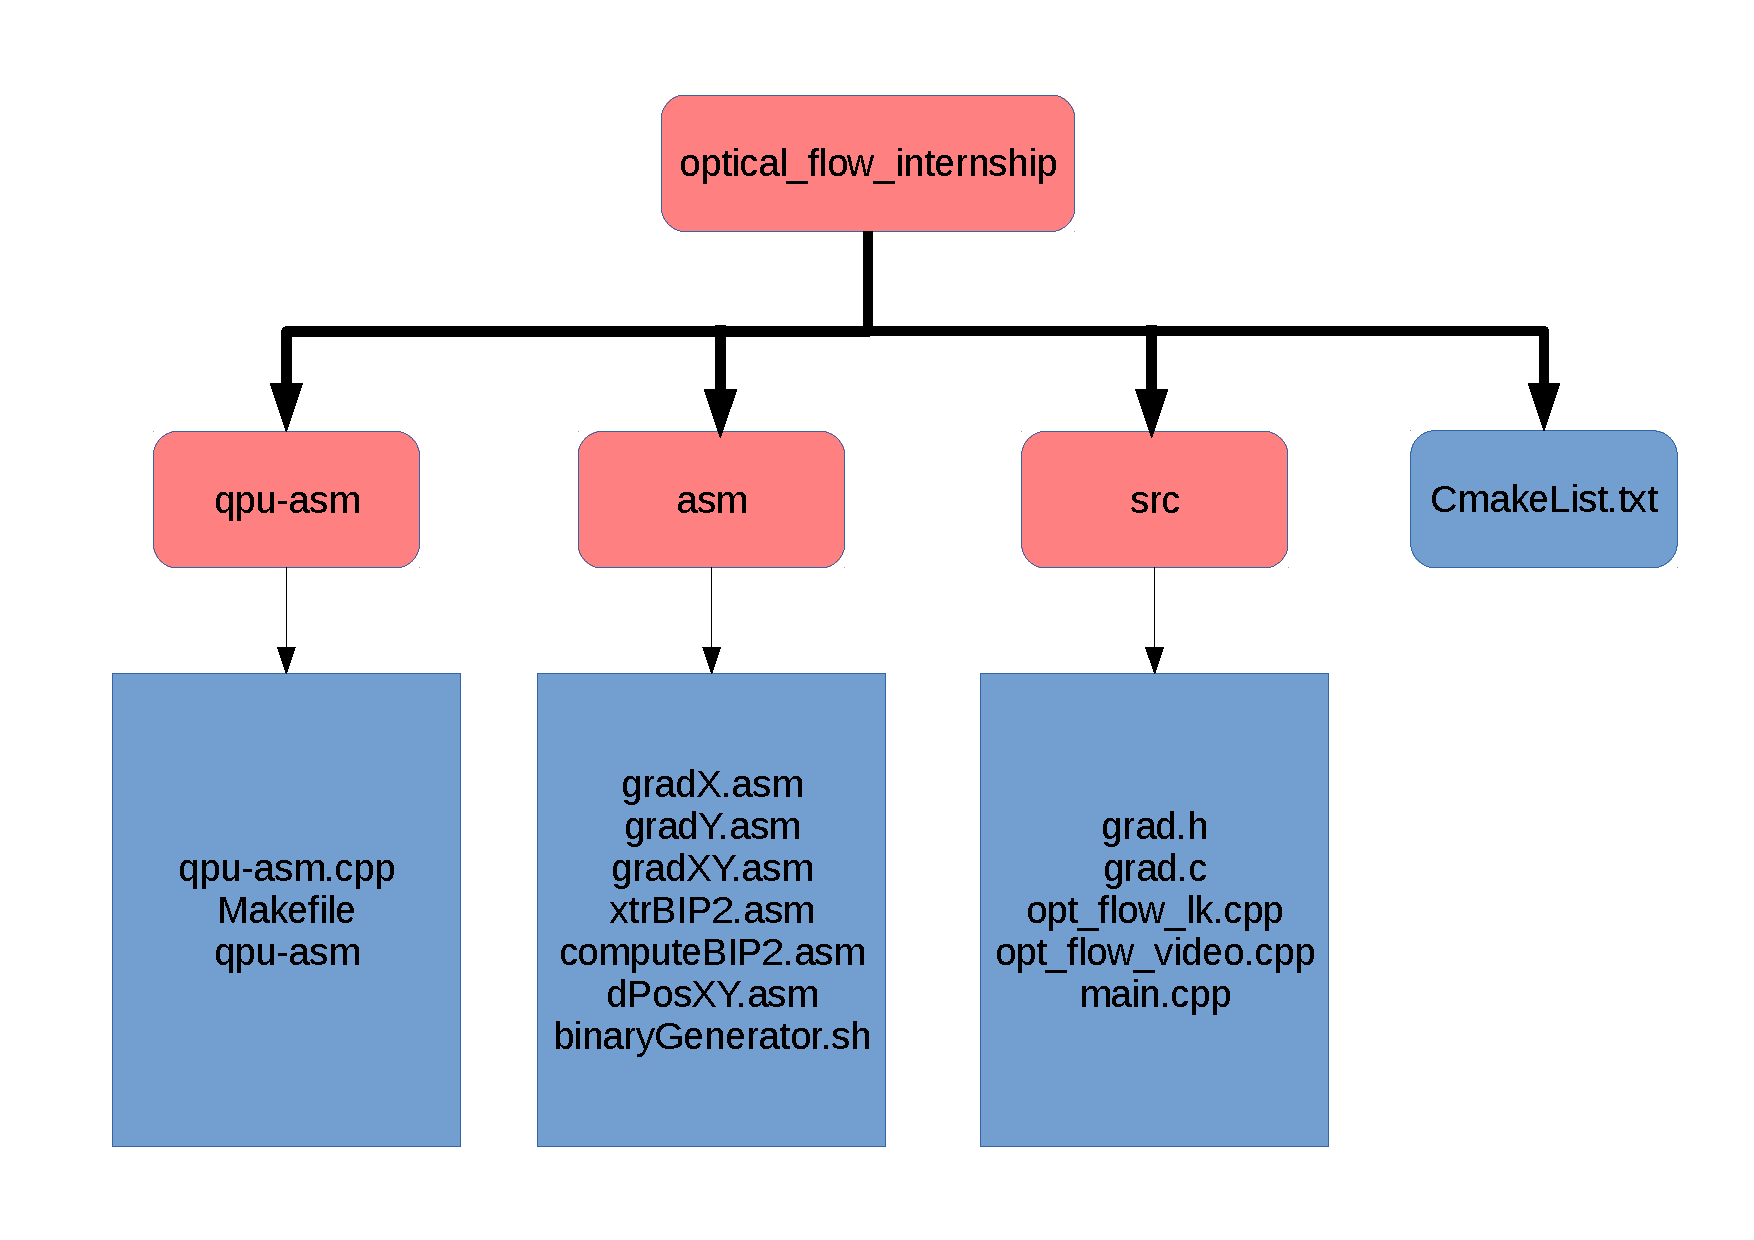
\includegraphics[width=0.8\textwidth]{optFlowArchitecture}
\caption{\file{optical\_flow\_internship} project to test the homemade \api}
	\label{optFlowFig}
\end{figure}
\FloatBarrier

-- To integrate the \api{} I add the \file{qpu-asm} and \file{asm} directories to the existing \file{optical\_flow\_internship} project. I also add \file{grad.c} and \file{grad.c} to \file{src} directory. Finally I modified \file{opt\_flow\_lk.cpp}, \file{opt\_flow\_video.cpp} and \file{main.cpp} to be able to run \flow{} \code{code} on \vc.

-- \file{qpu-asm} is the \keyword{assembly parser} written be Pete \textsc{Warden}: Chapter~\ref{Chapter2}.

-- \file{asm} directories contains all the \code{code-to-execute} on \vc. This code needs in several \file{.asm} file written in \option{assembly language}. Moreover, there is \file{binaryGenerator.sh} file, a \code{shell script} that translate all \file{.asm} files into \file{.bin} files that \vc{} will understands (Appendice~\ref{AppendixG}).

-- \file{grad.h} and \file{grad.c} are the \keyword{GPU} driver. In these file there are functions to:
\begin{itemize}
	\item initialize GPU
	\item map \ram{} memory and bind \emph{ARM Virtual Addresses} \& \emph{VC CPU Bus Addresses}
	\item copy code and data in the \ram
	\item send code pointers and variables called \uni{}s to the \qpu{}s
	\item get back results
\end{itemize}


-- To run the project:
\lstset{language=make,caption={},label=}
\begin{lstlisting}
cd qpu-asm && make
cd asm && ./binaryGenerator.sh
mkdir build && cd build
cmake..
make
sudo ./optical_flow_internship /path_to_video_sample
\end{lstlisting}


\subsection{main.cpp}

\lstset{style=CStyle,caption={main.cpp},label=mainList}
\begin{lstlisting}
#include <iostream>
#include <stdio.h>
#include <opencv2/opencv.hpp>
#include ``opt_flow_process_directory_video.hpp''


extern ``C'' {
	#include ``grad.h''
	#include ``mailbox.h''
}


using namespace std;

int main(int argc, char** argv)
{
	grad_init();

	OptFlowProcessDirectoryVideo directory;
	directory.video_to_process.set_use_opencv_lk(false);
	directory.video_to_process.set_use_lk_gpu(true);

	directory.process_all_videos_folder(argv[1]);

	freeMemory();
}
\end{lstlisting}

-- After including \file{mailbox.h} and \file{grad.h}, \code{grad\_init()} does allmost every step from listings~\ref{map},~\ref{init},~\ref{arithmetic},~\ref{transfer}:
\begin{itemize}
	\item initialize \qpu{}s: \code{qpu\_enable()}
	\item map \ram{} and bind \emph{ARM Virtual Addresses} with \emph{VC CPU Bus Addresses} with \code{mapmem()}
	\item copy code and data in \ram
	\item send code pointers and some wanted \uni{}s
\end{itemize}

This function doesn't invoke \code{execute\_qpu()}. This will be done inside \code{compute\_lk\_gpu()}. Also, we choose between \emph{OpenCV} and \keyword{GPU} by passing \option{true} or \option{false} parameters. Finally we call \code{freeMemory()} to disable \qpu{}s and flush \ram.


\subsection{opt\_flow\_lk.cpp}

This file contains the \code{compute\_lk\_gpu()} function. The source code of the function is written in Appendice~\ref{AppendixG}.

This function is divided in 3 parts:
\begin{itemize}
	\item \option{pre-processing} -- Sections ~\ref{parameters}, ~\ref{fctParams}
		\begin{itemize}
			\item provides $\textcolor{blue}{firstFrame_{0,0}}$ from \file{cv::Mat prev\_gray} -- \code{frame1\_float\_ptr} inside function
			\item provides $\textcolor{red}{secondFrame_{0,0}}$  from \file{cv::Mat gray} -- \code{frame2\_float\_ptr}
			\item provides \file{int} $featuresArray[2][30]$ -- \code{features\_static }
		\end{itemize}
	\item \option{GPU} -- Section~\ref{GPUconclusion}
		\begin{itemize}
			\item invokes functions from \file{grad.c}
			\item copies $\textcolor{blue}{firstFrame}$, $\textcolor{red}{secondFrame}$ and $features\_static$ in \ram
			\item processes first frame to get gradient values -- Section~\ref{gradientProcessing}
			\item runs the displacement algorithm to get 30 $(d_{x}, d_{y})$ values -- Figure~\ref{algoFig}
			\item gives back results to \cpu in \option{float} \code{d\_pos[2*30]} array
		\end{itemize}
	\item \option{post-processing}
		\begin{itemize}
			\item values from \code{d\_pos[2*30]} are pushed into an \emph{OpenCV} object for the rest of \keyword{CMT} algorithm
		\end{itemize}
\end{itemize}

\subsection{GPU driver: driver.h - driver.c}
I followed the same method as in the previous part~\ref{GPUconclusion} invoke GPU.

My driver (grad.c) will:
\begin{itemize}
	\item initialize \qpu{}s
	\item map the \ram
	\item copy code and data (frames 1 and 2 and featuresArray) in \ram
	\item send code pointer and \uni{}s
	\item get back the results
\end{itemize}

\subsection{asm: code-to-execute on \vc}
